\documentclass{standalone}
\usepackage{tikz}
\usetikzlibrary{patterns, positioning}


\begin{document}
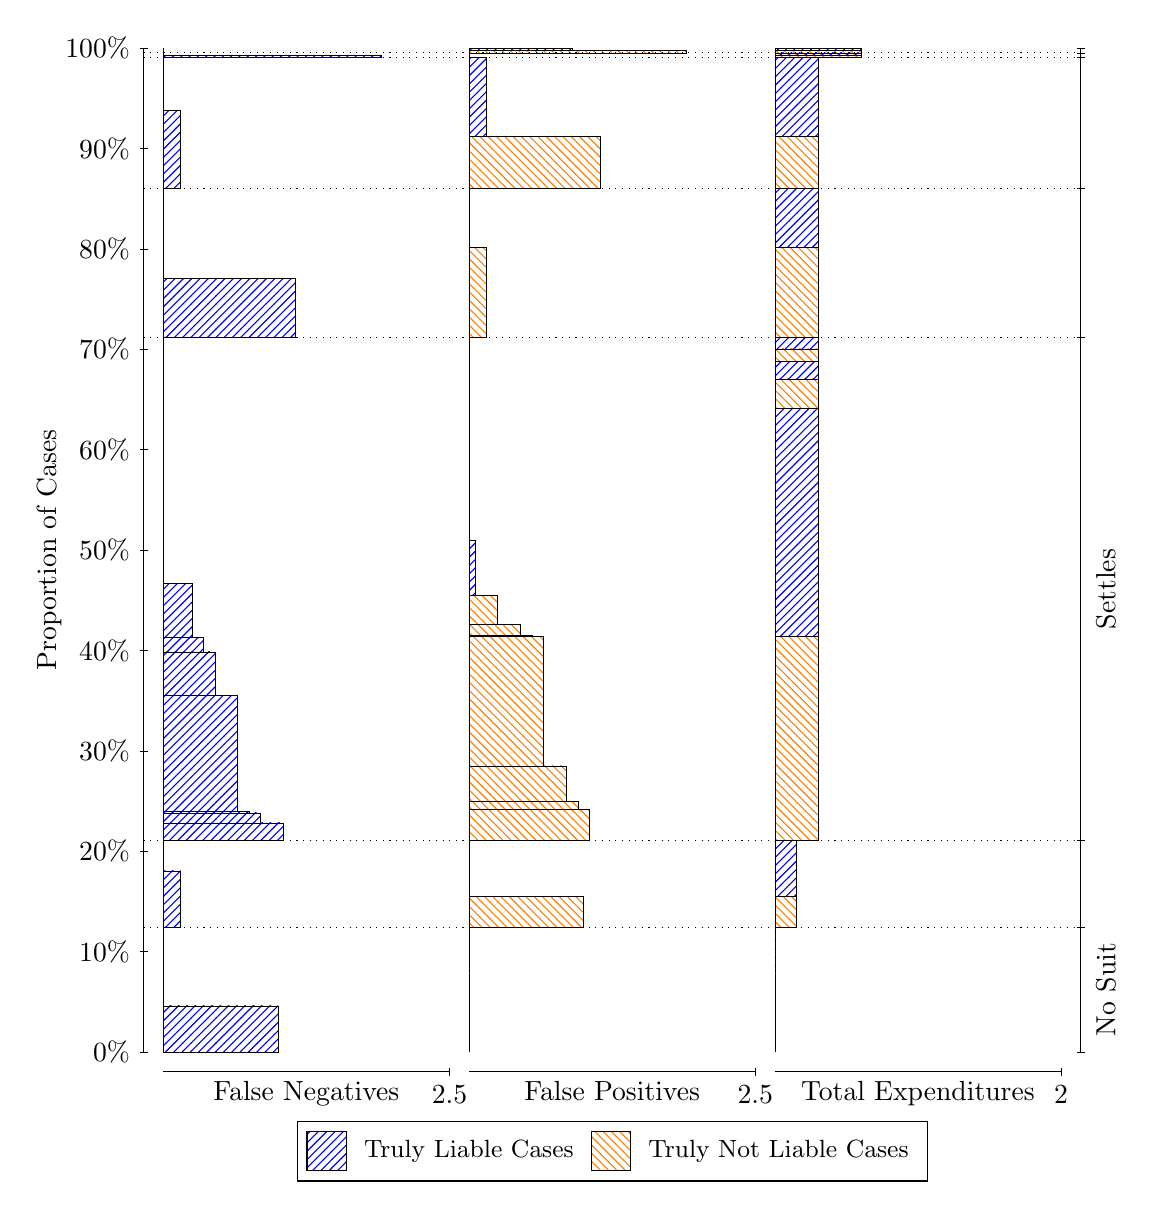
\begin{tikzpicture}
\draw[black, very thin] (1.5,1.75) -- (1.5,14.5);
\node[rotate=90, text=black, anchor=center] at (0.3, 8.125) {Proportion of Cases};
\draw[black, very thin] (1.45,1.75) -- (1.55,1.75);
\node[text=black, anchor=east] at (1.45, 1.75) {0\%};
\draw[black, very thin] (1.45,3.025) -- (1.55,3.025);
\node[text=black, anchor=east] at (1.45, 3.025) {10\%};
\draw[black, very thin] (1.45,4.3) -- (1.55,4.3);
\node[text=black, anchor=east] at (1.45, 4.3) {20\%};
\draw[black, very thin] (1.45,5.575) -- (1.55,5.575);
\node[text=black, anchor=east] at (1.45, 5.575) {30\%};
\draw[black, very thin] (1.45,6.85) -- (1.55,6.85);
\node[text=black, anchor=east] at (1.45, 6.85) {40\%};
\draw[black, very thin] (1.45,8.125) -- (1.55,8.125);
\node[text=black, anchor=east] at (1.45, 8.125) {50\%};
\draw[black, very thin] (1.45,9.4) -- (1.55,9.4);
\node[text=black, anchor=east] at (1.45, 9.4) {60\%};
\draw[black, very thin] (1.45,10.675) -- (1.55,10.675);
\node[text=black, anchor=east] at (1.45, 10.675) {70\%};
\draw[black, very thin] (1.45,11.95) -- (1.55,11.95);
\node[text=black, anchor=east] at (1.45, 11.95) {80\%};
\draw[black, very thin] (1.45,13.225) -- (1.55,13.225);
\node[text=black, anchor=east] at (1.45, 13.225) {90\%};
\draw[black, very thin] (1.45,14.5) -- (1.55,14.5);
\node[text=black, anchor=east] at (1.45, 14.5) {100\%};

\draw[black, very thin] (13.4,1.75) -- (13.4,14.5);
\draw[black, very thin] (13.35,1.75) -- (13.45,1.75);
\node[anchor=west] at (13.35, 1.75) {};
\draw[black, very thin] (13.35,3.3333) -- (13.45,3.3333);
\node[anchor=west] at (13.35, 3.3333) {};
\draw[black, very thin] (13.35,4.4377) -- (13.45,4.4377);
\node[anchor=west] at (13.35, 4.4377) {};
\draw[black, very thin] (13.35,10.821) -- (13.45,10.821);
\node[anchor=west] at (13.35, 10.821) {};
\draw[black, very thin] (13.35,12.716) -- (13.45,12.716);
\node[anchor=west] at (13.35, 12.716) {};
\draw[black, very thin] (13.35,14.378) -- (13.45,14.378);
\node[anchor=west] at (13.35, 14.378) {};
\draw[black, very thin] (13.35,14.439) -- (13.45,14.439);
\node[anchor=west] at (13.35, 14.439) {};
\draw[black, very thin] (13.35,14.5) -- (13.45,14.5);
\node[anchor=west] at (13.35, 14.5) {};

\draw[black, very thin, pattern color=blue, pattern=north east lines] (1.75,1.75) rectangle (3.2033,2.3353);
\draw[black, very thin, pattern color=orange, pattern=north west lines] (1.75,2.3353) rectangle (1.75,3.3333);
\draw[black, very thin, pattern color=blue, pattern=north east lines] (1.75,3.3333) rectangle (1.968,4.0485);
\draw[black, very thin, pattern color=orange, pattern=north west lines] (1.75,4.0485) rectangle (1.75,4.4377);
\draw[black, very thin, pattern color=blue, pattern=north east lines] (1.75,4.4377) rectangle (3.276,4.6608);
\draw[black, very thin, pattern color=blue, pattern=north east lines] (1.75,4.6608) rectangle (2.9853,4.786);
\draw[black, very thin, pattern color=blue, pattern=north east lines] (1.75,4.786) rectangle (2.84,4.8029);
\draw[black, very thin, pattern color=blue, pattern=north east lines] (1.75,4.8029) rectangle (2.6947,6.278);
\draw[black, very thin, pattern color=blue, pattern=north east lines] (1.75,6.278) rectangle (2.404,6.831);
\draw[black, very thin, pattern color=blue, pattern=north east lines] (1.75,6.831) rectangle (2.2587,7.0146);
\draw[black, very thin, pattern color=blue, pattern=north east lines] (1.75,7.0146) rectangle (2.1133,7.7059);
\draw[black, very thin, pattern color=orange, pattern=north west lines] (1.75,7.7059) rectangle (1.75,10.821);
\draw[black, very thin, pattern color=blue, pattern=north east lines] (1.75,10.821) rectangle (3.4213,11.571);
\draw[black, very thin, pattern color=orange, pattern=north west lines] (1.75,11.571) rectangle (1.75,12.716);
\draw[black, very thin, pattern color=blue, pattern=north east lines] (1.75,12.716) rectangle (1.968,13.712);
\draw[black, very thin, pattern color=orange, pattern=north west lines] (1.75,13.712) rectangle (1.75,14.378);
\draw[black, very thin, pattern color=blue, pattern=north east lines] (1.75,14.378) rectangle (4.5113,14.405);
\draw[black, very thin, pattern color=orange, pattern=north west lines] (1.75,14.405) rectangle (1.75,14.439);
\draw[black, very thin, pattern color=orange, pattern=north west lines] (1.75,14.439) rectangle (1.75,14.466);
\draw[black, very thin, pattern color=blue, pattern=north east lines] (1.75,14.466) rectangle (1.75,14.5);
\draw[black, very thin, pattern color=orange, pattern=north west lines] (5.6333,1.75) rectangle (5.6333,2.748);
\draw[black, very thin, pattern color=blue, pattern=north east lines] (5.6333,2.748) rectangle (5.6333,3.3333);
\draw[black, very thin, pattern color=orange, pattern=north west lines] (5.6333,3.3333) rectangle (7.0867,3.7225);
\draw[black, very thin, pattern color=blue, pattern=north east lines] (5.6333,3.7225) rectangle (5.6333,4.4377);
\draw[black, very thin, pattern color=orange, pattern=north west lines] (5.6333,4.4377) rectangle (7.1593,4.8294);
\draw[black, very thin, pattern color=orange, pattern=north west lines] (5.6333,4.8294) rectangle (7.014,4.9338);
\draw[black, very thin, pattern color=orange, pattern=north west lines] (5.6333,4.9338) rectangle (6.8687,5.3824);
\draw[black, very thin, pattern color=orange, pattern=north west lines] (5.6333,5.3824) rectangle (6.578,7.0233);
\draw[black, very thin, pattern color=orange, pattern=north west lines] (5.6333,7.0233) rectangle (6.4327,7.0414);
\draw[black, very thin, pattern color=orange, pattern=north west lines] (5.6333,7.0414) rectangle (6.2873,7.1824);
\draw[black, very thin, pattern color=orange, pattern=north west lines] (5.6333,7.1824) rectangle (5.9967,7.5528);
\draw[black, very thin, pattern color=blue, pattern=north east lines] (5.6333,7.5528) rectangle (5.706,8.2441);
\draw[black, very thin, pattern color=blue, pattern=north east lines] (5.6333,8.2441) rectangle (5.6333,10.821);
\draw[black, very thin, pattern color=orange, pattern=north west lines] (5.6333,10.821) rectangle (5.8513,11.967);
\draw[black, very thin, pattern color=blue, pattern=north east lines] (5.6333,11.967) rectangle (5.6333,12.716);
\draw[black, very thin, pattern color=orange, pattern=north west lines] (5.6333,12.716) rectangle (7.3047,13.382);
\draw[black, very thin, pattern color=blue, pattern=north east lines] (5.6333,13.382) rectangle (5.8513,14.378);
\draw[black, very thin, pattern color=orange, pattern=north west lines] (5.6333,14.378) rectangle (5.6333,14.412);
\draw[black, very thin, pattern color=blue, pattern=north east lines] (5.6333,14.412) rectangle (5.6333,14.439);
\draw[black, very thin, pattern color=orange, pattern=north west lines] (5.6333,14.439) rectangle (8.3947,14.466);
\draw[black, very thin, pattern color=blue, pattern=north east lines] (5.6333,14.466) rectangle (6.9413,14.5);
\draw[black, very thin, pattern color=orange, pattern=north west lines] (9.5167,1.75) rectangle (9.5167,2.748);
\draw[black, very thin, pattern color=blue, pattern=north east lines] (9.5167,2.748) rectangle (9.5167,3.3333);
\draw[black, very thin, pattern color=orange, pattern=north west lines] (9.5167,3.3333) rectangle (9.7892,3.7225);
\draw[black, very thin, pattern color=blue, pattern=north east lines] (9.5167,3.7225) rectangle (9.7892,4.4377);
\draw[black, very thin, pattern color=orange, pattern=north west lines] (9.5167,4.4377) rectangle (10.062,7.0233);
\draw[black, very thin, pattern color=blue, pattern=north east lines] (9.5167,7.0233) rectangle (10.062,9.9262);
\draw[black, very thin, pattern color=orange, pattern=north west lines] (9.5167,9.9262) rectangle (10.062,10.297);
\draw[black, very thin, pattern color=blue, pattern=north east lines] (9.5167,10.297) rectangle (10.062,10.52);
\draw[black, very thin, pattern color=orange, pattern=north west lines] (9.5167,10.52) rectangle (10.062,10.679);
\draw[black, very thin, pattern color=blue, pattern=north east lines] (9.5167,10.679) rectangle (10.062,10.821);
\draw[black, very thin, pattern color=orange, pattern=north west lines] (9.5167,10.821) rectangle (10.062,11.967);
\draw[black, very thin, pattern color=blue, pattern=north east lines] (9.5167,11.967) rectangle (10.062,12.716);
\draw[black, very thin, pattern color=orange, pattern=north west lines] (9.5167,12.716) rectangle (10.062,13.382);
\draw[black, very thin, pattern color=blue, pattern=north east lines] (9.5167,13.382) rectangle (10.062,14.378);
\draw[black, very thin, pattern color=orange, pattern=north west lines] (9.5167,14.378) rectangle (10.607,14.412);
\draw[black, very thin, pattern color=blue, pattern=north east lines] (9.5167,14.412) rectangle (10.607,14.439);
\draw[black, very thin, pattern color=orange, pattern=north west lines] (9.5167,14.439) rectangle (10.607,14.466);
\draw[black, very thin, pattern color=blue, pattern=north east lines] (9.5167,14.466) rectangle (10.607,14.5);
\draw[black, dotted] (1.5,3.3333) -- (13.4,3.3333);
\draw[black, dotted] (1.5,4.4377) -- (13.4,4.4377);
\draw[black, dotted] (1.5,10.821) -- (13.4,10.821);
\draw[black, dotted] (1.5,12.716) -- (13.4,12.716);
\draw[black, dotted] (1.5,14.378) -- (13.4,14.378);
\draw[black, dotted] (1.5,14.439) -- (13.4,14.439);
\draw[black, very thin] (1.75,1.5) -- (5.3833,1.5);
\node[text=black, anchor=north] at (3.5667, 1.5) {False Negatives};
\draw[black, very thin] (5.3833,1.45) -- (5.3833,1.55);
\node[text=black, anchor=north] at (5.3833, 1.45) {2.5};

\draw[black, very thin] (5.6333,1.5) -- (9.2667,1.5);
\node[text=black, anchor=north] at (7.45, 1.5) {False Positives};
\draw[black, very thin] (9.2667,1.45) -- (9.2667,1.55);
\node[text=black, anchor=north] at (9.2667, 1.45) {2.5};

\draw[black, very thin] (9.5167,1.5) -- (13.15,1.5);
\node[text=black, anchor=north] at (11.333, 1.5) {Total Expenditures};
\draw[black, very thin] (13.15,1.45) -- (13.15,1.55);
\node[text=black, anchor=north] at (13.15, 1.45) {2};

\node[text=black, centered, rotate=90] at (13.72, 2.5417) {No Suit};

\node[text=black, centered, rotate=90] at (13.72, 7.6294) {Settles};





\draw (7.449999999999999,1.5) node[draw=none] (baseCoordinate) {};
\begin{scope}[align=center]
        \matrix[scale=0.5, draw=black, below=0.5cm of baseCoordinate, nodes={draw}, column sep=0.1cm]{
            \node[rectangle, draw, minimum width=0.5cm, minimum height=0.5cm, pattern color=blue, pattern=north east lines] {}; &
            \node[draw=none, font=\small, text=black] (B) {Truly Liable Cases}; &
            \node[rectangle, draw, minimum width=0.5cm, minimum height=0.5cm, pattern color=orange, pattern=north west lines] {}; &
            \node[draw=none, font=\small, text=black] (B) {Truly Not Liable Cases}; \\
            };
\end{scope}

\end{tikzpicture}
\end{document}